%
% dreieck3d1.tex
%
% (c) 2021 Prof Dr Andreas Müller, OST Ostschweizer Fachhochschule
%
\documentclass[tikz]{standalone}
\usepackage{times}
\usepackage{amsmath}
\usepackage{txfonts}
\usepackage[utf8]{inputenc}
\usepackage{graphics}
\usetikzlibrary{arrows,intersections,math}
\usepackage{ifthen}
\begin{document}

%
% common.tex -- gemeinsame definition
%
% (c) 2017 Prof Dr Andreas Müller, Hochschule Rapperswil
%
%
% packages.tex -- packages required by the paper sturmliouville
%
% (c) 2019 Prof Dr Andreas Müller, Hochschule Rapperswil
%

% if your paper needs special packages, add package commands as in the
% following example
%\usepackage{packagename}


%
% common.tex -- gemeinsame definition
%
% (c) 2017 Prof Dr Andreas Müller, Hochschule Rapperswil
%
%
% packages.tex -- packages required by the paper sturmliouville
%
% (c) 2019 Prof Dr Andreas Müller, Hochschule Rapperswil
%

% if your paper needs special packages, add package commands as in the
% following example
%\usepackage{packagename}


%
% common.tex -- gemeinsame definition
%
% (c) 2017 Prof Dr Andreas Müller, Hochschule Rapperswil
%
\input{../common/packages.tex}
\input{../common/common.tex}
\mode<beamer>{%
\usetheme[hideothersubsections,hidetitle]{Hannover}
}
\beamertemplatenavigationsymbolsempty
\title[Navigation]{Sphärische Navigation}
\author[E.~E.~und~M.~K.]{Enez Erdem und Marc Kühne}
\date[]{16.~Mai 2022}
\newboolean{presentation}


\mode<beamer>{%
\usetheme[hideothersubsections,hidetitle]{Hannover}
}
\beamertemplatenavigationsymbolsempty
\title[Navigation]{Sphärische Navigation}
\author[E.~E.~und~M.~K.]{Enez Erdem und Marc Kühne}
\date[]{16.~Mai 2022}
\newboolean{presentation}


\mode<beamer>{%
\usetheme[hideothersubsections,hidetitle]{Hannover}
}
\beamertemplatenavigationsymbolsempty
\title[Navigation]{Sphärische Navigation}
\author[E.~E.~und~M.~K.]{Enez Erdem und Marc Kühne}
\date[]{16.~Mai 2022}
\newboolean{presentation}



\newboolean{showgrid}
\setboolean{showgrid}{false}
\def\breite{4}
\def\hoehe{4}

\begin{tikzpicture}[>=latex,thick]

% Povray Bild
\node at (0,0) {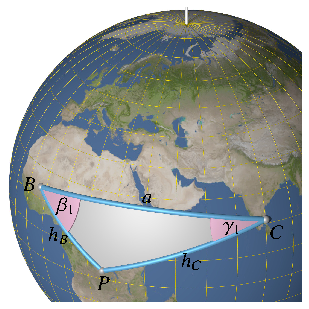
\includegraphics[width=8cm]{position3.jpg}};

% Gitter
\ifthenelse{\boolean{showgrid}}{
\draw[step=0.1,line width=0.1pt] (-\breite,-\hoehe) grid (\breite, \hoehe);
\draw[step=0.5,line width=0.4pt] (-\breite,-\hoehe) grid (\breite, \hoehe);
\draw                            (-\breite,-\hoehe) grid (\breite, \hoehe);
\fill (0,0) circle[radius=0.05];
}{}

\labelB
\labelC
\labelP

\labela

\labelhb
\labelhc

\labelbetaone
\labelgammaone

\end{tikzpicture}

\end{document}

